\documentclass{ctexart}

%\usepackage{pgfkeys}% included in tikz package
\usepackage{tikz}

\begin{document}

\section{Introduction(87.1)}

% store code: <key>/.code=<handler>
\pgfkeys{/message text/.code=The message is '#1'.}
% execute code stored for <key>
\pgfkeys{/message text=hi!}
\pgfkeys{/message text=hello!}

% <key> with more than one parameter
\pgfkeys{/message text/.code 2 args=The messages are '#1' and '#2'.}
\pgfkeys{/message text={hello}{world}}

% <key> with default value
\pgfkeys{/message text/.code=(#1)}
\pgfkeys{/message text/.default=hello world}
\pgfkeys{/message text}\par
\pgfkeys{/message text=hi,/message text}

% .style 设定 key-value list
\pgfkeys{/foo/.code=(a:#1)}
\pgfkeys{/bar/.code=(b:#1)}
\pgfkeys{/foobar/.style={/foo=foo,/bar=bar}}
\pgfkeys{/foobar}\par
\pgfkeys{/foobar/.style={/foo=foo,/bar=bar,/foo=#1}}
\pgfkeys{/foobar=hello}\par
\pgfkeys{/foobar/.style 2 args={/foo=#1,/bar=#2}}
\pgfkeys{/foobar={hello}{world}}

% 定义 keys
\pgfkeys{/foo/line width/.code=line width:#1\par}
\pgfkeys{/foo/draw/.code=draw:#1\par}
% Setup keys
\pgfkeys{/foo/.style=/foo/.cd}
\pgfkeys{foo,line width=1cm,draw=red}%先切换至 /foo,再设置 keys

\section{The Key Tree(87.2)}

% 类似 \def
\pgfkeyssetvalue{/foo family/bar key}{Hello, world!}
\pgfkeysvalueof{/foo family/bar key}

% 类似 \let
\def\helloworld{Hello, world!}
\pgfkeyslet{/foo family/bar key}{\helloworld}
\pgfkeysvalueof{/foo family/bar key}

% 将 key 赋给一个宏
\pgfkeyssetvalue{/foo family/bar key}{Hello, world!}
\pgfkeysgetvalue{/foo family/bar key}{\foo}
\foo

% 测试 key 是否被定义
\pgfkeysifdefined{/foo family/bar key}{已定义}{未定义}\par
\pgfkeysifdefined{/foo family/foobar key}{已定义}{未定义}

\section{Setting Keys(87.3)}

% pattern
\pgfkeysdefargs{/foo}{#1 and #2}{1:#1, 2:#2}
\pgfkeys{/foo=hello and world}

\section{Key Handlers(87.4)}

% .cd
\pgfkeys{/foo/color/.code=color:#1\par}
\pgfkeys{/foo/.cd,color=red}

% .is family
\pgfkeys{/foo/.is family}
\pgfkeys{foo,color=blue}

% .default
\pgfkeys{
  /foo/bgcolor/.code=bgcolor:#1\par,
  /foo/bgcolor/.default=purple
}
\pgfkeys{/foo/bgcolor}
\pgfkeys{/foo/.cd,bgcolor=red}

% .code 2 args
\pgfkeys{/page size/.code 2 args={paper height:#2, paper width:#1}}
\pgfkeys{/page size={30cm}{20cm}}

% .code n args n = 0 to 9
\pgfkeys{/foo/.code n args={3}{1:#1,2:#2,3:#3}}
\pgfkeys{/foo={A}{B}{C}}

% .code args={<argument pattern>}{<code>}
\pgfkeys{/foo/.code args={#1 and #2}{1:#1,2:#2}}
\pgfkeys{/foo=A B and B and C}

% defining styles
% 要执行的代码
\pgfkeys{/par indent/.code={\parindent=#1}}
% 定义 style
\pgfkeys{/no indent/.style={/par indent=0pt}}
\pgfkeys{/normal indent/.style={/par indent=2em}}
\par\pgfkeys{/no indent}
Lorem ipsum dolor sit amet, consectetur adipiscing elit, sed do eiusmod tempor incididunt ut labore et dolore magna aliqua.
\par\pgfkeys{/normal indent}
Lorem ipsum dolor sit amet, consectetur adipiscing elit, sed do eiusmod tempor incididunt ut labore et dolore magna aliqua.

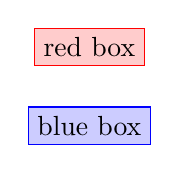
\begin{tikzpicture}[outline/.style={draw=#1,fill=#1!20}]
  \node[outline=red] at (0,0) {red box};
  \node[outline=blue] at (0,-1) {blue box};
\end{tikzpicture}

% .style 2 args
\pgfkeys{
  /paper height/.code=paper height:#1\par,
  /paper width/.code=paper width:#1\par,
  /page size/.style 2 args={/paper height=#1,/paper width=#2}
}
\pgfkeys{/page size={30cm}{20cm}}

% .style args={<argument pattern>}{<key list>}
\pgfkeys{
  /paper height/.code=paper height:#1\par,
  /paper width/.code=paper width:#1\par,
  /page size/.style args={#1 and #2}{/paper height=#1,/paper width=#2}
}
\pgfkeys{/page size=30cm and 20cm}

% .store in
\pgfkeys{/foo/.store in=\text}
\pgfkeys{/foo={Hello,world!}}% 含有逗号, 需要使用{}
\text

\end{document}